\section{Programmazione multicore}
L'utilizzo di più thread si adatta naturalmente ai sistemi multicore, ma non solo, essa può trovare delle applicazioni anche in sistemi con un solo processore.

\subsection{Concorrenza}
La Concorrenza è l'esecuzione di più attività contemporaneamente, questo può essere ottenuto con un sistema multicore, oppure tramite uno scheduling efficiente dei cicli di un singolo processore.

\spacer
La concorrenza permette, almeno dal punto di vista dell'utente, di eseguire più processi contemporaneamente anche se questo può non essere vero.

Questo si ottiene tramite una grande quantità di \textit{context switch} da parte della CPU, che dedica ad ogni task una quantità di tempo infinitesimale.

Risulta quindi particolarmente importante scegliere correttamente le task che possono essere eseguite contemporaneamente e come sincronizzare.

\begin{figure}[H]
    \centering
    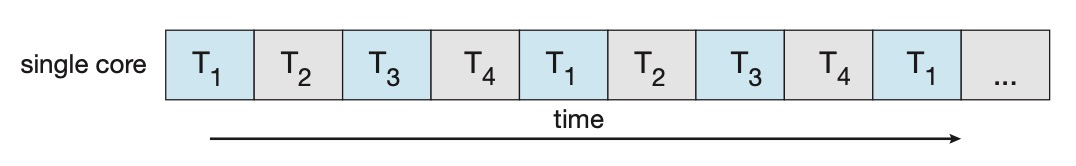
\includegraphics[width=0.65\linewidth]{assets/concorrenza.jpg}
    \caption{Concorrenza su un singolo processore}
\end{figure}

\subsection{Parallelismo}
Il parallelismo invece è la semplice esecuzione due o più task contemporaneamente. I due thread non devono necessariamente lavorare alla risoluzione dello stesso problema.
\begin{figure}[H]
    \centering
    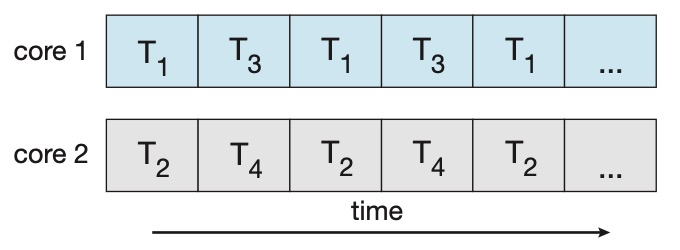
\includegraphics[width=0.45\linewidth]{assets/parallelismo.jpg}
    \caption{Parallelismo su due processori}
\end{figure}

\spacer
Il parallelismo può essere implementato in vari modi:
\begin{itemize}
    \item \textbf{Parallelismo dei dati:}

          La stessa operazione viene eseguita contemporaneamente su processori diversi su segmenti diversi dei dati. (es. per analizzare 10 ore di registrazione, divido in elementi da 1 ora ciascuno)

    \item \textbf{Parallelismo delle task:}

          Significa distribuire i threads tra più processori, ogni thread esegue un'operazione differente. I thread possono lavorare sugli stessi dati, ma non è necessario.
\end{itemize}

\begin{figure}[H]
    \centering
    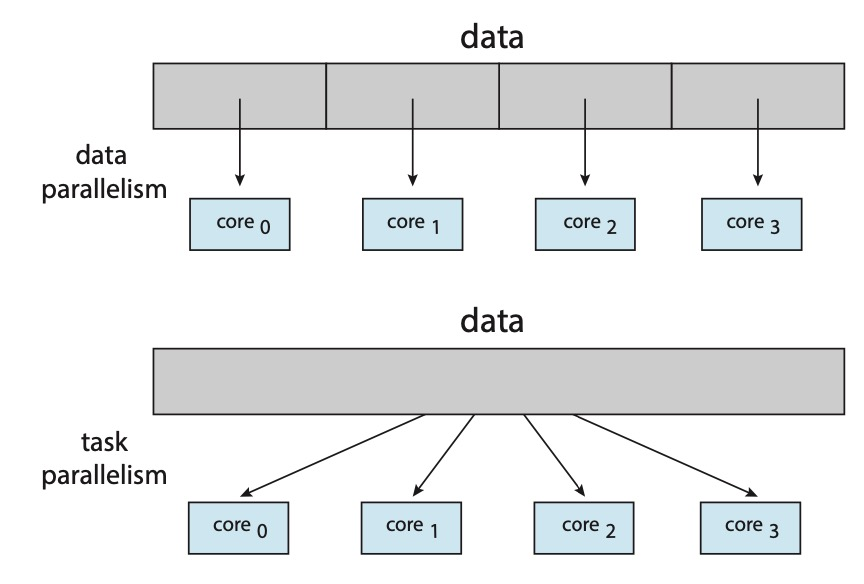
\includegraphics[width=0.45\linewidth]{assets/data-task-parallelism.jpg}
\end{figure}
